%!TEX root = index.tex
\chapter{Experiments}
\label{section:testing}

\red{TODO: intro}

\section{Comparison of scheduling algorithms on single runway}
\label{section:1rwy-alternating}

This test compares the performance of implemented scheduling algorithms. The scenario contains twelve flights with alternating weight class landing on one runway arriving in close succession. This scenario should be particularly demanding to be scheduled optimally because the alternation in weight classes make it sensitive to the order in which the slots are scheduled.

\begin{table}[h]
  \centering
\begin{tabular}{ | l | c | r | r | }
\hline
Flight id	& Weight class	& Appearance on screen & Estimated arrival time	\\
\hline
01M	& MEDIUM	& 17:36	& 42:30	\\
02J	& JUMBO		& 19:24	& 42:29	\\
03J	& JUMBO		& 19:00	& 44:15	\\
04M	& MEDIUM	& 22:00	& 44:49	\\
05M	& MEDIUM	& 21:36	& 46:30	\\
06J	& JUMBO		& 23:24	& 46:29	\\
07J	& JUMBO		& 23:00	& 48:15	\\
08M	& MEDIUM	& 26:00	& 48:49	\\
09M	& MEDIUM	& 25:36	& 50:30	\\
10J	& JUMBO		& 27:24	& 50:29	\\
11J	& JUMBO		& 27:00	& 52:15	\\
12M	& MEDIUM	& 30:00	& 52:49	\\
\hline
\end{tabular}
  \caption{Configuration of the test scenario}
  \label{tab:config1}
\end{table}

Table \ref{tab:config1} shows the configuration of the test scenario. For the \texttt{JUMBO} category the Airbus A380-800 was used and the \texttt{MEDIUM} category was represented by Boeing 737. Airplanes headed to the airport from two separate streams to prevent possible violation of separation in en-route sectors the planes fly from.

\begin{figure}[h]
    \centering
    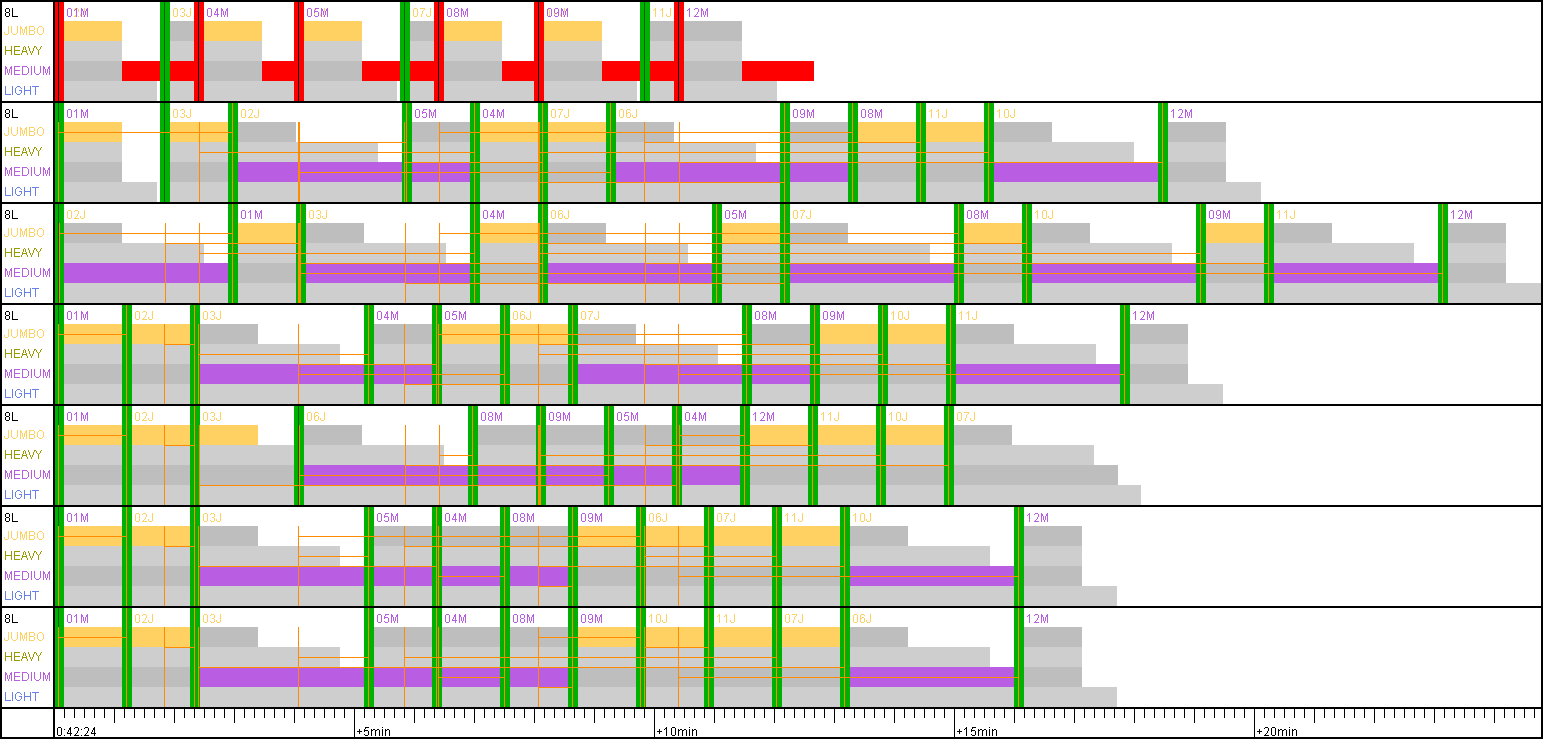
\includegraphics[width=\textwidth]{figures/1rwy-alternating.png}
    \caption{Result of planning with different algorithms on single runway}
    \label{fig:1rwy-alternating}
\end{figure}

The resulting plans are shown in Figure \ref{fig:1rwy-alternating}. The first row shows the result of {\em Algorithm~1} which places the slots in the exact time the arrival was estimated. It demonstrates how many collision would occur if no planning was present and serves as the lower bound on the total plan time.

The plans generated by {\em Algorithm~2} and {\em Algorithm~3} are identical in this case and are depicted in the second row. The slots are ordered in the same succession the corresponding aircraft appeared on the controller's screen. The reason the plans are identical is that the stream of arriving planes is very dense and there are no voids present between the aircraft the {\em Algorithm~3} would utilize to produce better schedule than {\em Algorithm~2}.

Third and fourth rows show the results of both versions of {\em Algorithm~4}. The third row contains the plan generated by the simple version of the algorithm, that keeps the order of aircraft's expected time of arrival. In this instance the algorithm produced the poorest result with the longest overall time as well as longest maximal and total delays. This is due to the specific configuration of the test scenario that alternates between weight classes. The second version doesn't rigorously keep the order of estimated arrival but tries to locally minimize the delays and therefore produces much better result.

The last three rows contain plans generated by the three versions of {\em Algorithm~5}. Each one shows optimal plan according to selected criterion. The one in the fifth row has the shortest total makespan. The plan in sixth row has the shortest maximal delay of a slot in the plan. And the last plan has minimal sum of delay of all slots. Note, that the last two plans are very similar and even have the same total length but the order of the slots determines whether the solution minimizes one or the other criterion.

\subsection{Makespan}

\begin{figure}[h]
    \centering
    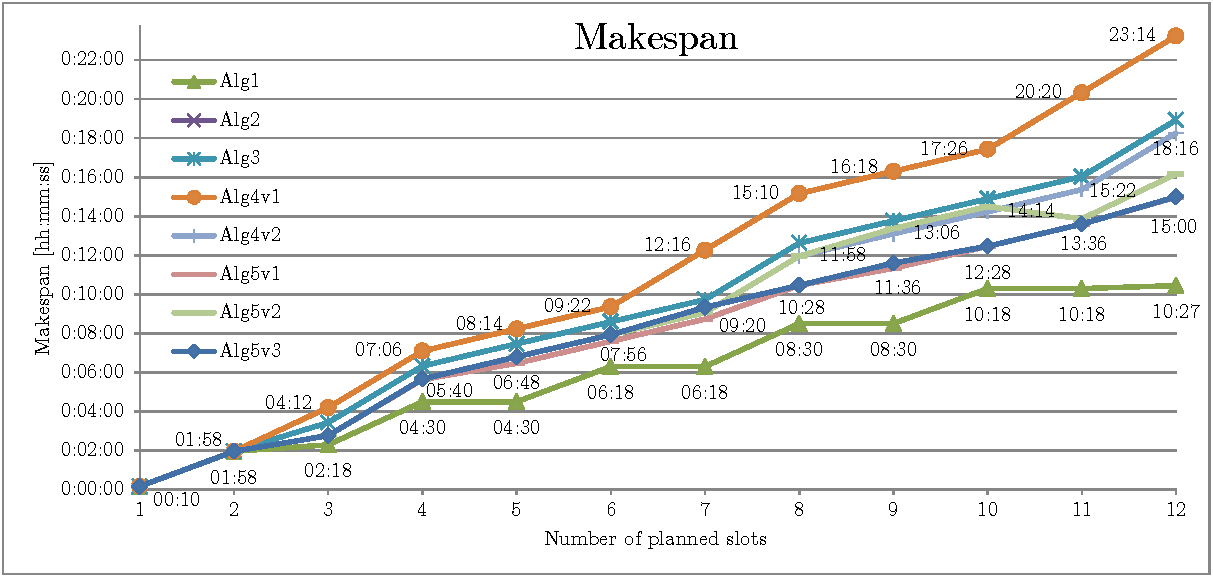
\includegraphics[width=\textwidth]{graphs/1rwy-alternating-makespan.pdf}
    \caption{Graph of makespan for plans created with different algorithms on single runway}
    \label{graph:1rwy-alternating-makespan}
\end{figure}

The obvious criterion by which the quality of a plan can be determined is the total duration of the schedule, also called makespan. The shorter the plan is, the better, because all the planes will in total land in the shortest possible time. In reality this criterion is problematic, because the flow of airplanes to the airport is infinite, only the density changes in time. But even so, this criterion can give a notion of the quality of immediate plan.

Makespan times in the progress of planning are shown in Graph \ref{graph:1rwy-alternating-makespan}. The result given by {\em Algorithm~1} is a lower bound that is given by the configuration of the testing scenario, no plans can be shorter than this value. The longest plans are generated by {\em Algorithm~4v1}. Plan with minimal makespan is generated by {\em Algorithm~5v1}, with {\em Algorithm~5v3} having very similar results (the values for 12 planned slots differ by less than one second) and {\em Algorithm~5v2} also being close. The results given by {\em Algorithm~4v2} are still near optimum with plans 22\% longer at most. {\em Algorithm~2} and {\em Algorithm~3} produce identical, fairly good plans.

\subsection{Maximal delay}

\begin{figure}[h]
    \centering
    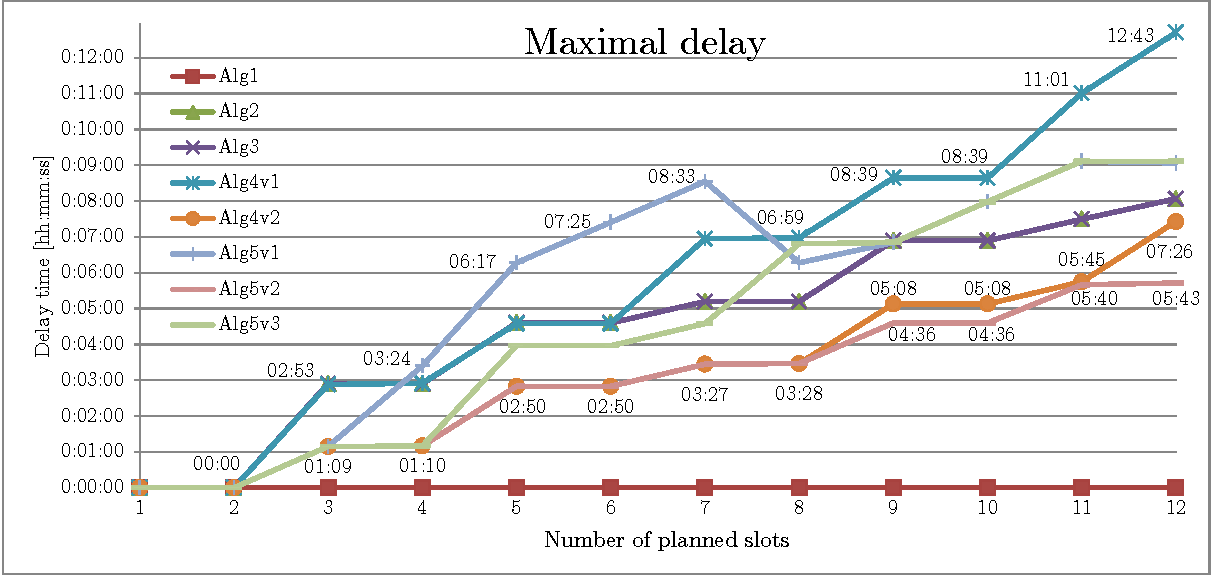
\includegraphics[width=\textwidth]{graphs/1rwy-alternating-maximal-delay.pdf}
    \caption{Graph of maximal delay for plans created with different algorithms on single runway}
    \label{graph:1rwy-alternating-maximal-delay}
\end{figure}

Another criterion that can describe the quality of a runway plan is the maximal delay among all slots. Obviously the smaller the delay is, the better the plan is. This criterion criterion can be used to prevent the situation in which one plane would give the priority to all others and would wait until its supply of fuel is depleted. The sum of all delays can be small, but the fact that the critical delay time for one aircraft was exceeded renders such plan potentially dangerous.

Graph \ref{graph:1rwy-alternating-maximal-delay} shows the development of values of this criterion during the planning. The optimal value for the final plan is 5 minutes and 43 seconds and is achieved by {\em Algorithm~5v2}. {\em Algorithm~4v1} has the poorest performance with the value of 12:43. {\em Algorithm~5v1} optimizes the total makespan and in order to do that it can delay some slots by a significant amount of time. This can lead to high maximal delay values as shown here for plans with 4 – 7 slots. {\em Algorithm~4v2} performs very well with its result at or very near the optimal value. For the final plan the maximal delay for this algorithm is 1 minute 43 second longer than the optimal value.

\subsection{Total delay}

\begin{figure}[h]
    \centering
    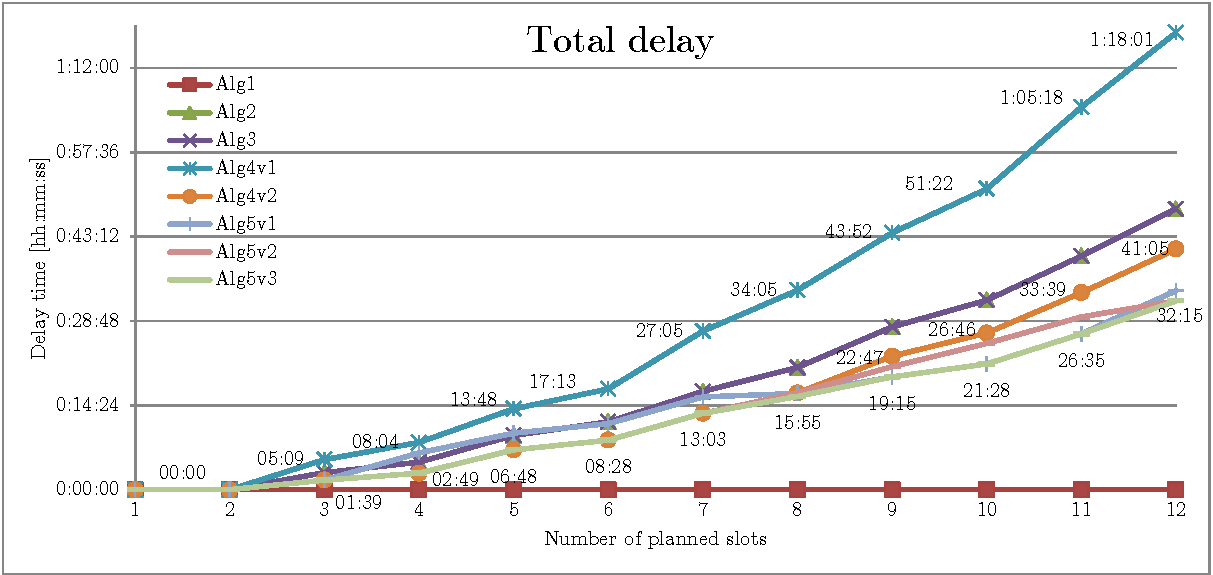
\includegraphics[width=\textwidth]{graphs/1rwy-alternating-total-delay.pdf}
    \caption{Graph of total delay for plans created with different algorithms on single runway}
    \label{graph:1rwy-alternating-total-delay}
\end{figure}

The sum of all slot delays is another way to measure runway plan's quality. It describes the total time wasted on waiting in the terminal area. It is also linked to the total amount of fuel burnt during the waiting. Both time and used amount of fuel affect the costs of the flight.

The total delay times in the progress of planning are shown in Graph \ref{graph:1rwy-alternating-total-delay}. The poorest results are again given by {\em Algorithm~4v1} with the total delay more than 2.4 times the optimum. The optimal result is produced by {\em Algorithm~5v3} (32:25 for final plan) with other two versions of the {\em Algorithm~5} very near. {\em Algorithm~4v2} performs well with the total delay at 41:05 which is less than 30\% more than the optimum. {\em Algorithm~2} and {\em Algorithm~3} still perform good and could produce usable results but are not as good as {\em Algorithm~4v2}.

\subsection{Replanned slots}

\begin{figure}[h]
    \centering
    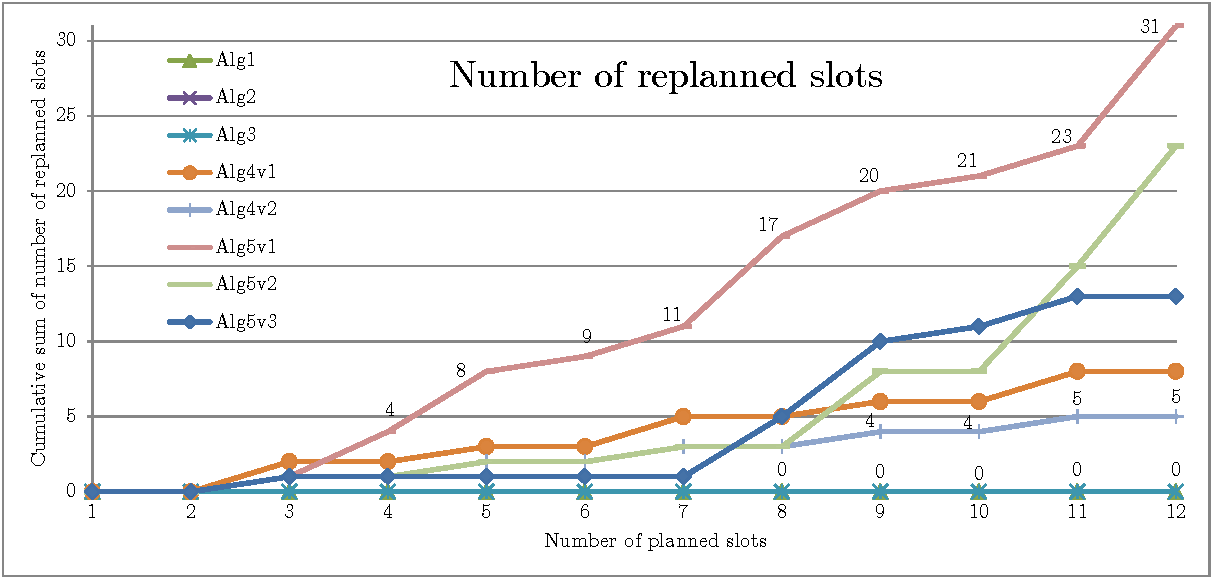
\includegraphics[width=\textwidth]{graphs/1rwy-alternating-replanned-slots.pdf}
    \caption{Graph of cumulative sum of replanned slots for plans created with different algorithms on single runway}
    \label{graph:1rwy-alternating-replanned-slots}
\end{figure}

The number of replanned slots shown in Graph \ref{graph:1rwy-alternating-replanned-slots} expresses how often the controller must interfere with the schedule of previously planned aircraft after a new one has been added to the plan. This criterion has a relation to the controllers workload, because he/she must contact each replanned aircraft and give the pilot updated instructions.

{\em Algorithm~1}, {\em Algorithm~2} and {\em Algorithm~3} place the new slots in a way that doesn't affect the previously planned and therefore don't cause the need to replan old slots. {\em Algorithm~4v2} with five replanned slots during the creation of final plan produces very good results according to the aforementioned criteria but is still undemanding of frequent replanning of old slots. All three versions of {\em Algorithm~5} have high numbers of replanned slots because the fat that they look for optimal solution causes them to change the plan significantly with each slot addition. This is especially true for {\em Algorithm~5v1} which minimizes the total makespan. Its 31 replanned slots during the creation of plan for 12 planes render it unusable for real world application.

\subsection{Conclusion}

{\em Algorithm~1} isn't intended for real-world use and it's performance is irrelevant. {\em Algorithm~2} and {\em Algorithm~3} behave identically in this scenario providing usable results in every measured aspect with the main advantage being that previously planned slots are fixed and there is no need to update the pilots instruction when new plane flies in. {\em Algorithm~4v1} performs poorly and doesn't handle the alternating weight classes well. On the other hand, similar {\em Algorithm~4v2} that adds the local optimization of delay, gives good results not too far from optimal solution with low number of slots being replanned. {\em Algorithm~5v1–3} obviously give the optimal result in the categories they are optimizing for but can have inferior results in other categories (e.g. versions 1 and 3 for maximal delay). The fact that the algorithms strive for the optimum result also means that these algorithms tend to replan previous slots often causing high workload for the controller. This and their computational complexity makes them unusable in real-world application.

\section{Real world flights on single runway}

The next test compared implemented scheduling algorithms on real-world air traffic. The test scenario contained 764 flights going through ZTL Center on 20th June 2013 between 12:00 a.m. and 6:00 p.m. All flights were arriving to runway \texttt{8L} of Atlanta airport. Moreover the wake separation minima were increased to minimum of 4 NM \red{minutes?} to make the arrival slots bigger and therefore the arriving flow of traffic relatively denser.

The flights were scheduled for approach using four algorithms. {\em Algorithm~1} was not used because it produces invalid plan with possible collisions. All three variants of {\em Algorithm~5} were also not used because their computational complexity makes them unsuitable for planning in real-world scenario with hundreds of flights.

\begin{table}[h]
  \centering
\begin{tabular}{|l|r|r|r|r|}
\hline
Scheduling algorithm & Makespan  & Maximal delay & Total delay & Updated slots \\
\hline
Algorithm 2   & 22:22:25  & 4:25:13 & 53d 16:08:22 & 0    \\
Algorithm 3   & 22:20:12  & 4:23:00 & 52d 13:56:08 & 0    \\
Algorithm 4v1 & 22:18:54  & 4:15:23 & 51d 21:34:16 & 2038 \\
Algorithm 4v2 & 22:19:18  & 4:15:47 & 51d 21:42:57 & 2025 \\
\hline
\end{tabular}
  \caption{Results of different scheduling algorithms for dense real-world traffic on single runway}
  \label{tab:1rwy-real}
\end{table}

The results of the test are shown in Table \ref{tab:1rwy-real}. Because only the actual, final plan is studied in this case, only the results for entire plan with all slots are shown, not their progress during the planning.

The lower bound on makespan given by {\em Algorithm~1} defined by the configuration of the test scenario is 18:05:23, no plan can be shorter than that. The actual plans were about 4 hours longer. The differences between the algorithms are small with the longest makespan no more than 4 minutes longer than the shortest.

Differences between maximal delays of the schedules are slightly bigger with the interval between smallest and biggest value spanning 10 minutes. The values for both variants of {\em Algorithm~4} are virtually identical. In real-world scenario, delay of more than four hours would certainly cause the plane to deplete its fuel reserve and crash since the commercial flights are in usual conditions required to have 30 minutes reserve of fuel for holding at the destination airport.\cite[Chapter 4]{annex6} In this case the extreme value is caused by dense traffic, restricting the arrivals to a single runway and enlarging the wake turbulence separation minima to almost twice the usual value.

The total delay results show how even small differences of the algorithms performance can have significant impact when large number of airplanes is affected. {\em Algorithm~4v1} generated schedule in which the total waiting time is 1 day 18 hours and 34 minutes smaller than in schedule made by {\em Algorithm~2}. More than 42 hours worth of fuel and passenger time is very significant saving. The results of both variants of {\em Algorithm~4} are again virtually same, the total delays differ only by 8 minutes and 41 second (less than 0.012\%).

{\em Algorithm~2} and {\em 3} don't update slots once they're planned. The second version outperforms the first variant of {\em Algorithm~4} by 13 updated slots during the planning. The overall number of updates is fairly hight but with average 2.7 updates per plane not unrealistically demanding for the air traffic controller. Also with lower density of the traffic, this number would be lower.

In conclusion, this test shows that all four algorithms produce similar and usable results in scenarios with high density real-world traffic. The best results were planned by {\em Algorithm~4v1}. On the other hand, results by {\em Algorithm~4v2} were nearly identical and this algorithm is more robust in situations with alternating weight classes of the arriving airplanes as shown in previous test. Therefore {\em Algorithm~4v2} was selected to be used in further tests for planning on multiple runways.

\section{Planes with alternating weight class on multiple runways}

This test is aimed to compare the quality of different criteria for choosing which runway the plane should land on. The configuration is the same as in Test \ref{section:1rwy-alternating} with the exception that the planes don't land on single runway but on runways \texttt{8L} and \texttt{9R} on Atlanta airport. See Table \ref{tab:config1} for the configuration of flights in the scenario.

\begin{figure}[h]
    \centering
    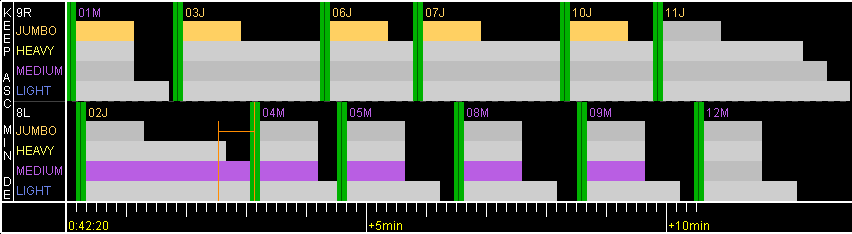
\includegraphics[width=\textwidth]{figures/2rwy-weight.png}
    \caption{Result of planning with different algorithms on multiple runways \red{update image}}
    \label{fig:2rwy-weight}
\end{figure}

The resulting plans are shown in Figure \ref{fig:2rwy-weight}. The first two rows show results of scheduling with makespan criterion on each runway and the second two rows show the plans generated by the remaining criteria since they produce identical results. Table \ref{tab:2rwy-alternating} contains measured values generated using different approaches. Each value is a sum of results from both runways. \red{TODO} The makespan criterion performs worse than the rest and even produces plan with longer sum of makespans which may seem paradoxical but is due to the fact the optimization is local and locally optimal solution for adding slots early on may prevent the algorithm to have optimal results while other slots are added to the plan later. \red{TODO}

\begin{table}[h]
  \centering
\begin{tabular}{|l|r|r|r|r|}
\hline
Scheduling criterion & Makespan  & Maximal delay & Total delay & Updated slots \\
\hline
Makespan      & 22:34  & 2:10 & 2:12 & 0 \\
Total delay   & 20:25  & 0:37 & 0:37 & 0 \\
Maximal delay & 20:25  & 0:37 & 0:37 & 0 \\
New slot ETA  & 20:25  & 0:37 & 0:37 & 0 \\
\hline
\end{tabular}
  \caption{Results of different scheduling criteria for flights with alternating weight classes on multiple runways}
  \label{tab:2rwy-alternating}
\end{table}

The addition of second runway to the test caused lower relative traffic density and the test therefore doesn't provide enough information to assess the quality of all the criteria for choosing runway. That is why following test comparing the criteria on real-world scenario was conducted.

\section{Real World Flights on Multiple Runways}

\red{TODO}


\red{TODO: sjednotit velikost pismen v nadpisech}

\section{Real World Flights With Miles In Trails}

\begin{figure}[h]
    \centering
    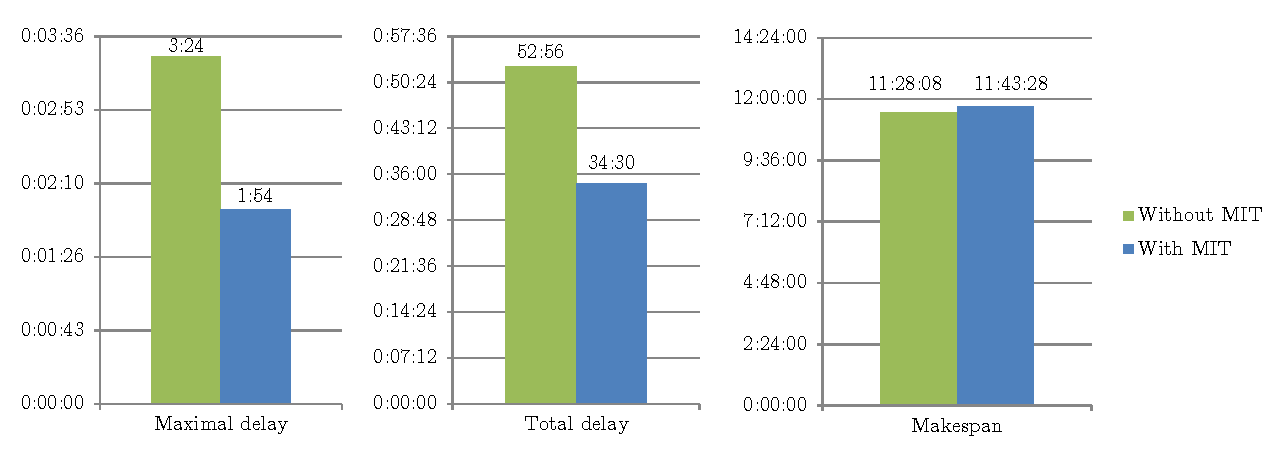
\includegraphics[width=\textwidth]{graphs/mit.pdf}
    \caption{\red{chart}}
    \label{graph:mit}
\end{figure}